\documentclass[a4paper,12pt]{article}
\usepackage[ukrainian,english]{babel}
\usepackage{ucs}
\usepackage[utf8]{inputenc}
\usepackage[T2A]{fontenc}
\usepackage{amsmath}
\usepackage{bigints}
\usepackage{amsfonts}
\usepackage{graphicx}
\usepackage{wrapfig}
\newcommand{\dx}{\textbf{d}x}
\newcommand{\dt}{\textbf{d}t}
\newcommand{\du}{\textbf{d}u}
\newcommand{\dv}{\textbf{d}v}
\newcommand{\dy}{\textbf{d}}
\newcommand{\arch}{\textrm{arcch}}
\newcommand{\arsh}{\textrm{arcsh}}
\newcommand{\dint}{\displaystyle\int}
\newcommand\tab[1][1cm]{\hspace*{#1}}
\makeatletter
\newcommand{\skipitems}[1]{%
  \addtocounter{\@enumctr}{#1}%
}
\makeatother
\usepackage[left=20mm, top=20mm, right=10mm, bottom=20mm, nohead, nofoot]{geometry}

\begin{document}

\title{Розрахункова Робота №4}
\author{ФІ-12 Бекешева Анастасія}
\maketitle
\newpage
\begin{enumerate}
	\item $\dint\arctan\sqrt{4x-1}\dx=\dint\arctan\sqrt{4x-1}\dy{(4x-1)}=x\arctan\sqrt{4x-1}-\\-\dfrac12\dint\dfrac{\dy(4x-1)}{\sqrt{4x-1}}=x\arctan\sqrt{4x-1}-\dfrac14\sqrt{4x-1}+c$
	\item $\dint\limits_{-2}^0(x^2-4)\cos3x\dx=\left|\begin{array}{ll}
		u=x^2-4&\dv=\cos3x\dx\\
		\du=2x\dx&v=\frac13\sin3x
	\end{array} \right|=\dfrac13(x^2-4)\sin3x\bigg|_{-2}^0-\\-\dfrac23\dint\limits_{-2}^0x\sin3x\dx=\left|\begin{array}{ll}
		u=x&\dv=\sin3x\dx\\\du=\dx&v=-\frac13\cos3x
	\end{array} \right|=-\dfrac23\left(-\dfrac13x\cos3x\bigg|_{-2}^0+\dfrac13\dint\limits_{-2}^0\cos3x\dx \right)=\\=-\dfrac23\left(-\dfrac23\cos6+\dfrac19\sin3x \right)=\dfrac49\cos6-\dfrac2{27}\sin6$
	\item $\dint\dfrac{1+\ln x}x\dx=\dint\dfrac\dx x+\dint\ln x\dy(\ln x)=\ln|x|+\frac12\ln^2x+c$
	\item $\dint\limits_0^1\dfrac{(x^2+1)\dx}{(x^3+3x+1)}=\left|\begin{array}{l}
		t=x^3+3x+1\\\dx=\dfrac1{3x^2+3}\dt
	\end{array} \right|=\dfrac13\dint\limits_0^1\dfrac\dt{t^2}=-\dfrac1{3t}=-\dfrac1{3(x^3+3x+1)}\bigg|_0^1=\dfrac4{15}$
	\item $\dint\dfrac{3x^3+1}{x^2-1}\dx=\dint\left(3x+\dfrac{3x+1}{(x-1)(x+1)} \right)\dx$ \textcircled{=}\\$\tab =\dfrac A{x-1}+\dfrac B{x+1}\\\tab A=\dfrac{3x+1}{x+1}\bigg|_{x=1}=2\\\tab B=\dfrac{3x+1}{x-1}\bigg|_{x=-1}=1\\$\textcircled{=} $\dint\left(3x+\dfrac{2}{x-1}+\dfrac{1}{x+1} \right)\dx=\dfrac32x^2+2\ln|x-1|+\ln|x+1|+c$
	\item $\dint\dfrac{x^3+6x^2+13x+8}{x(x+2)^3}\dx=$ \textcircled{=}\\$\tab =\dfrac Ax+\dfrac B{(x+2)^3}\\\tab A=\dfrac{x^3+6x^2+13x+8}{(x+2)^2}\bigg|_{x=0}=1\\\tab B=\dfrac{x^3+6x^2+13x+8}{x}\bigg|_{x=-2}=1\\$\textcircled{=} $\dint\left(\dfrac1x+\dfrac1{(x+2)^3} \right)\dx=\ln|x|-\dfrac1{2(x+2)^2}+c$
	\skipitems{1}
	\item $\dint\limits_0^{\frac\pi2}\dfrac{\cos x\dx}{2+\cos x}=\dint\limits_0^{\frac\pi2}\left(1-\dfrac2{\cos x+2} \right)\dx=x\bigg|_0^{\frac\pi2}-2\dint\dfrac1{\cos^2\frac x2(\tan^2\frac x2)+3}dx=\left|t=\dfrac{\tan\frac x2}{\sqrt3} \right|=\\=x\bigg|_0^{\frac\pi2}-\dfrac4{\sqrt3}\dint\dfrac1{t^2+1}\dt=x\bigg|_0^{\frac\pi2}-\dfrac4{\sqrt3}\arctan\left(\dfrac{\tan\frac x2}{\sqrt3}	\right)\bigg|_0^{\frac\pi2}=\dfrac\pi2-\dfrac{2\pi}{\sqrt{3^3}}$
	\skipitems{1}
	\item $\dint\limits_0^\pi2^4\sin^6x\cos^2x\dx=\dint\limits_0^\pi\sin^2x\left(2-\dfrac{1-\cos2x}2\right)\dx=\dint\limits_0^\pi\sin^22x\left(1-2\cos2x+\cos^2x\right)\dx=\\=\dint\limits_0^\pi\sin^22x\dx+2\dint\limits_0^\pi\sin^22x\cos x\dx+\dint\limits_0^\pi\sin^22x\cos^2x\dx=\dint\limits_0^\pi\dfrac12(1-\cos4x)\dx-\\-\dint\limits_0^\pi\sin^22x\dy(\sin2x)+\dint\limits_0^\pi\dfrac18(1-\cos8x)\dx=\dfrac12\left(x-\dfrac14\sin4x\right)+\dfrac13\sin^3x+\dfrac18\left(x-\dfrac18\sin8x \right)\bigg|_0^\pi=\\=\dfrac\pi2+0+\dfrac\pi8=\dfrac{5\pi}8$
	\item $\dint\limits_1^{64}\dfrac{1-\sqrt[6]x+2\sqrt[3]x}{x+2\sqrt[3]x+\sqrt[3]{x^4}}\dx=\left|\begin{array}{ll}
		t=\sqrt[6]x&x=t^6\\
		\dx=6t^5&\dt\\
		t_1=1&t_2=2
	\end{array} \right|=\dint_1^2\dfrac{1-t+2t^2}{t^6+2t^3+t^8}\cdot6t^5\dt=\\=6\dint_1^2\dfrac{2t^2-t+1}{t(t+1)(2t^2-t+1)}\dt=6\dint_1^2\dfrac{\dt}{t(t+1)}=6\dint\limits_1^2\left(\dfrac1t-\dfrac1{t+1} \right)\dt=6(\ln|t|-\ln|t+1|)\bigg|_1^2=\\=6(2\ln2-\ln3)=6\ln\dfrac43$
	\item $\dint\limits_0^1x^2\sqrt{1-x^2}=\left|\begin{array}{ll}
		x=\sin t\\\dx=\cos t&\dt\\
		t_1=0&t_2=\dfrac\pi2
	\end{array} \right|=\dint\limits_0^{\frac\pi2}\sin^2t\sqrt{1-\sin^2t}\cos t\dt=\dint\limits_0^{\frac\pi2}\sin^2t\cos^2t\dt=\\=\dfrac14\dint\limits_0^{\frac\pi2}\sin^2t\dt=\dfrac18\dint\limits_0^{\frac\pi2}\left(1-\cos4t\right)\dt=\dfrac18\left(t-\dfrac{\sin4t}4 \right)\bigg|_0^\frac\pi2=\dfrac18\left(\dfrac\pi2-0\right)=\dfrac{\pi}{16}$
	\item $\dint\dfrac{\sqrt[3]{1+\sqrt x}}{x\sqrt[3]{x^2}}\dx=\dint x^{-\frac32}(x^{-\frac12}+1)^{\frac13}\dx=\left|\begin{array}{l}
		t=x^{-\frac12}+1\\\dt=-\dfrac12x^{-\frac32}\dx
	\end{array} \right|=-2\dint t^{\frac13}dt=-\dfrac32t^{\frac43}=\\=-\dfrac32\sqrt{\left(1+\dfrac1{\sqrt x} \right)}+c$
	\item $y=x\sqrt{9-x^2},\>y=0\>(0\leq x\leq 3)\\\begin{array}{l}
		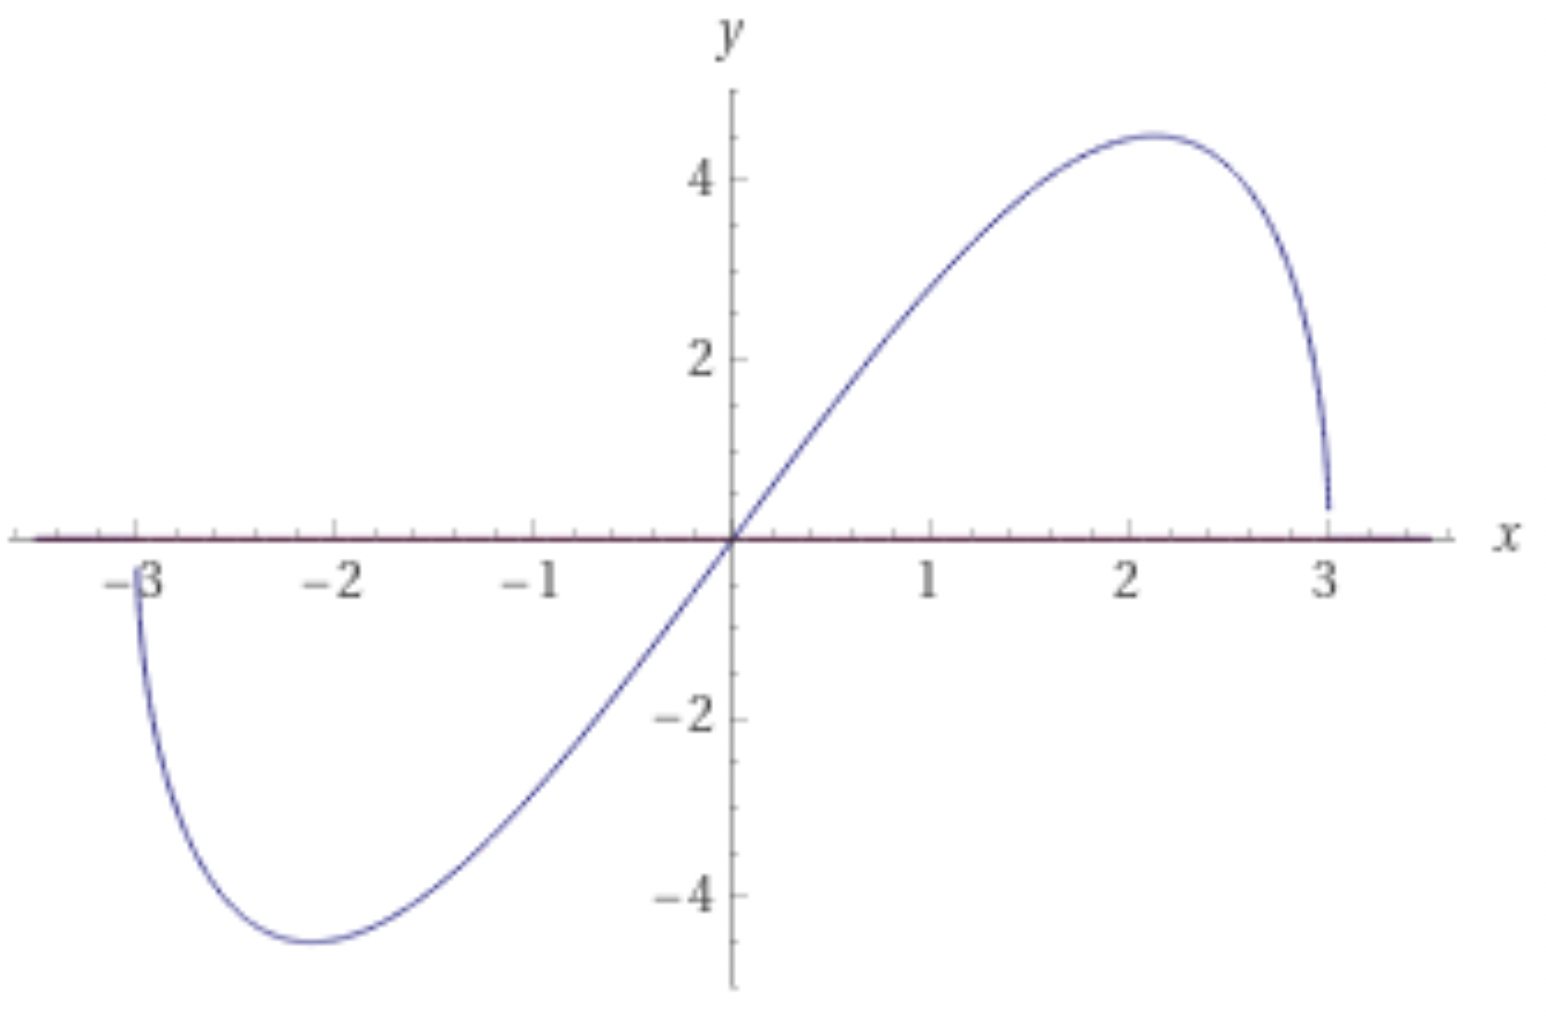
\includegraphics[width=5cm]{cl14}
	\end{array}\begin{array}{l}
		S=\dint\limits_0^3y\dx=\dint\limits_0^3x\sqrt{9-x^2}=\left|\begin{array}{ll}t=9-x^2&\dt=-2x\dx\\t_1=9&t_2=0 \end{array} \right|=\\=-\dint\limits_9^0\dfrac{\sqrt{t}}2\dx=-\dfrac16t^{\frac32}\bigg|_9^0=\dfrac{27}3-0=9
	\end{array}$
	\item $\left\{\begin{array}{l}
		x=\sqrt2\cos t\\y=2\sqrt2\sin t
	\end{array}\right.,y=2\>(y\geq2)\\\begin{array}{l}
		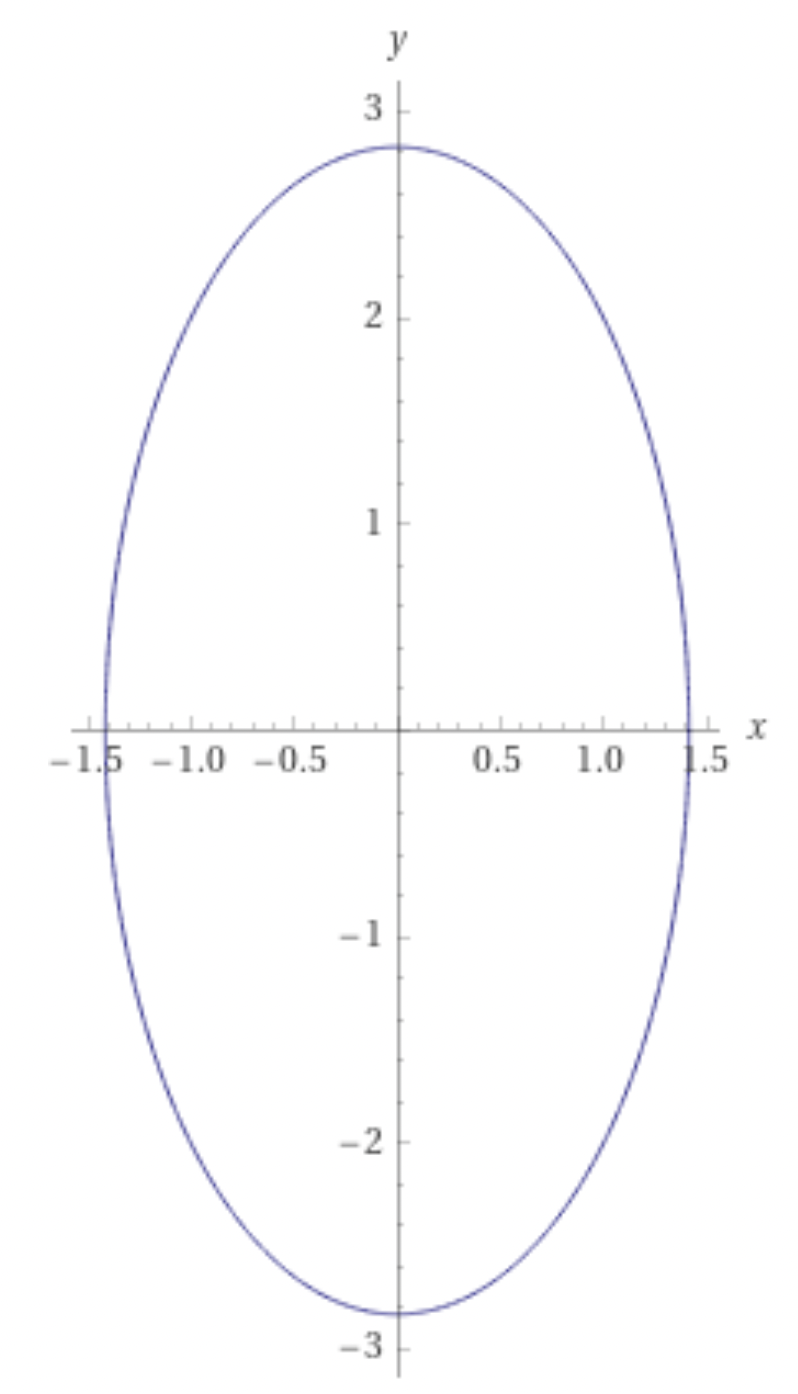
\includegraphics[height=4cm]{cl15}
	\end{array}\begin{array}{l}
		2\sqrt2\sin t\geq2\Rightarrow t\in\left[\dfrac\pi4, \dfrac{3\pi}4\right]\\S=\dint\limits_\frac\pi4^\frac{3\pi}42\sqrt2\sin t(-\sqrt2\sin t)\dt-2\cdot2=2\dint\limits_\frac\pi4^\frac{3\pi}4(1-\cos2t)\dt-4=\\=2\left(1-\dfrac12\sin2t\right)\bigg|_\frac\pi4^\frac{3\pi}4=\pi-2
	\end{array}$
	\item $r=\cos2\varphi\\\begin{array}{l}
		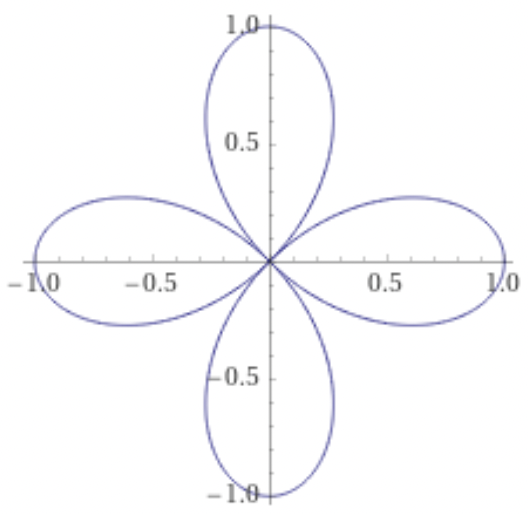
\includegraphics[width=5cm]{cl16_1}
	\end{array}\begin{array}{l}
		T=\pi,r=\cos2\varphi\geq0\Rightarrow\varphi\in\left[-\dfrac\pi4,\dfrac\pi4\right]\\S=2\left(\dfrac12\dint\limits_0^\frac\pi4 r^2\dy\varphi\right)=\dint\limits_0^\frac\pi4\cos^22\varphi\dy\varphi=\dfrac12\dint\limits_0^\frac\pi4(1+\cos4\varphi)\dy\varphi=\\=\dfrac12\left(\varphi+\dfrac14\sin4\varphi\right)\bigg|_0^\frac\pi4=\dfrac\pi8
	\end{array}$
	\item $y=\dfrac{x^2}4-\dfrac{\ln x}2,1\leq x\leq 2\\\begin{array}{l}
		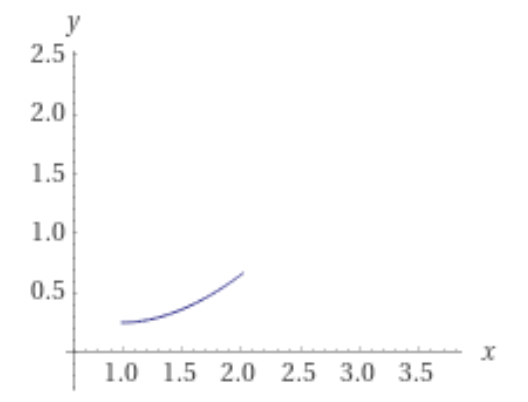
\includegraphics[height=4cm]{cl17}
	\end{array}\begin{array}{l}
		l=\dint\limits_1^2\sqrt{1+\dfrac{(x^2-1)^2}{4x^2}}\dx=\dint\limits_1^2\dfrac{x^2+1}{2x}\dx=\dfrac12\dint\limits_1^2\left(x+\dfrac1x \right)\dx=\\
		=\dfrac12\left(\dfrac{x^2}2+\ln|x| \right)\bigg|_1^2=\dfrac12\left(\dfrac32+\ln2\right)
	\end{array}$
	\item $\left\{\begin{array}{l}
		x=3(2\cos t-\cos2t)\\
		y=3(2\sin t-\sin2t)
	\end{array} \right.,0\leq t\leq2\pi\\\begin{array}{l}
		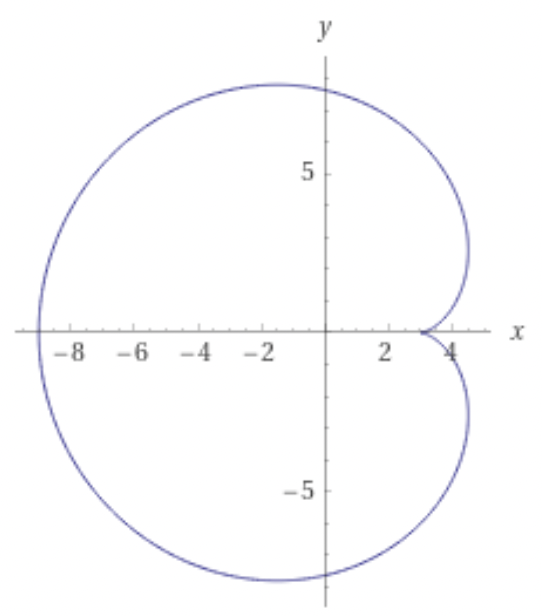
\includegraphics[width=5cm]{cl18}
	\end{array}\begin{array}{l}
		l=\dint\limits_0^\frac\pi2\sqrt{9(-2\sin t+2\sin t)^2+9(2\cos t-\cos2t)^2}\dt=\\=6\dint\limits_0^\frac\pi2\sqrt{2-2(\sin t\sin2t+\cos t\cos2t}\dt=6\dint\limits_0^\frac\pi2\sqrt{2-2\cos t}\dt=\\=6\dint\limits_0^\frac\pi2\sqrt{4\sin^2\dfrac t2}dt=12\dint\limits_0^\frac\pi2\sin\dfrac t2\dt=-24\cos\dfrac t2\bigg|_0^\frac\pi2=48
	\end{array}$
	\skipitems{1}
	\item $z=x^2+4y^2,z=2\\\begin{array}{l}
		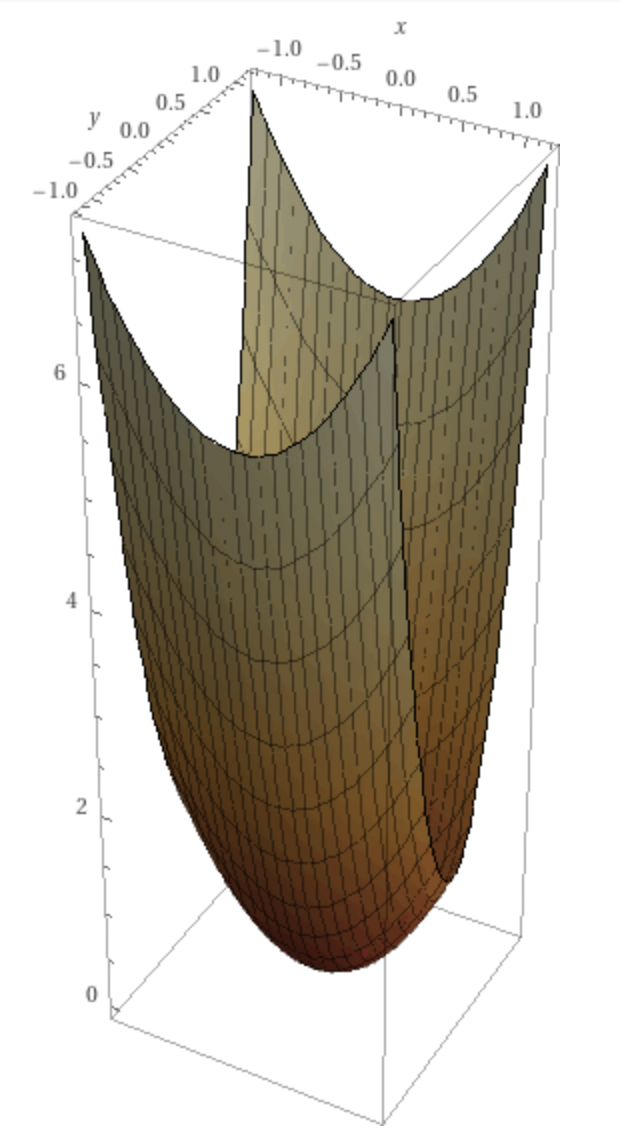
\includegraphics[width=3cm]{cl20}
	\end{array}\begin{array}{l}
		\dfrac{x^2}z+\dfrac{4y^2}z=1\Rightarrow a=\sqrt z,\>b=\dfrac{\sqrt z}2\Rightarrow S=\pi ab=\dfrac\pi2 z\\V=\dint\limits_0^2S(z)\dy z=\dfrac\pi2\dint\limits_0^2Sz\dy z=\dfrac\pi2\left(\dfrac{z^2}2 \right)\bigg|_0^2=\pi
	\end{array}$

\end{enumerate}




\end{document}